The \acrfull{RL}-based exploration of myopic transition pathways can require thousands of runs to converge. To reduce the computational burden and maximise this exploration, the learning phase of the agent could start on the monthly model before being refined on the one with an hourly time-resolution, the so-called transfer learning \cite{mann2013directed}.  Even though averaging time series of end-use demands and renewable productions brings some discrepancies (\ie faster emergence of local VRES and smaller electrification of the system), the main advantage of the monthly approach is its computational time, \ie couple of seconds versus 15 min for the hourly model (see Appendix \ref{app:mo_vs_td}). This section aims at comparing results from the learning process on the monthly model with the one on the hourly model. The monthly learning has been carried out by applying the same rules (see Section \ref{sec:RL:act_states_rew}). The purpose is to assess the capacity of the monthly model to be a good proxy of the hourly myopic transitions.

Considering the actions taken by the agent and their binding effect on the environment with a monthly resolution,  we see similar trends as in the hourly model (see Figure \ref{fig:app:Binding_constr_joss}). Limiting the consumption of coal is always binding where \gls{LFO} is ``naturally'' removed from the mix by the cost-minimisation. Where limiting the consumption of fossil gas has a major impact at the early stages, limiting the system emissions up to carbon-neutrality becomes more crucial at the end of the transition.

\begin{figure}[!htbp]
\centering
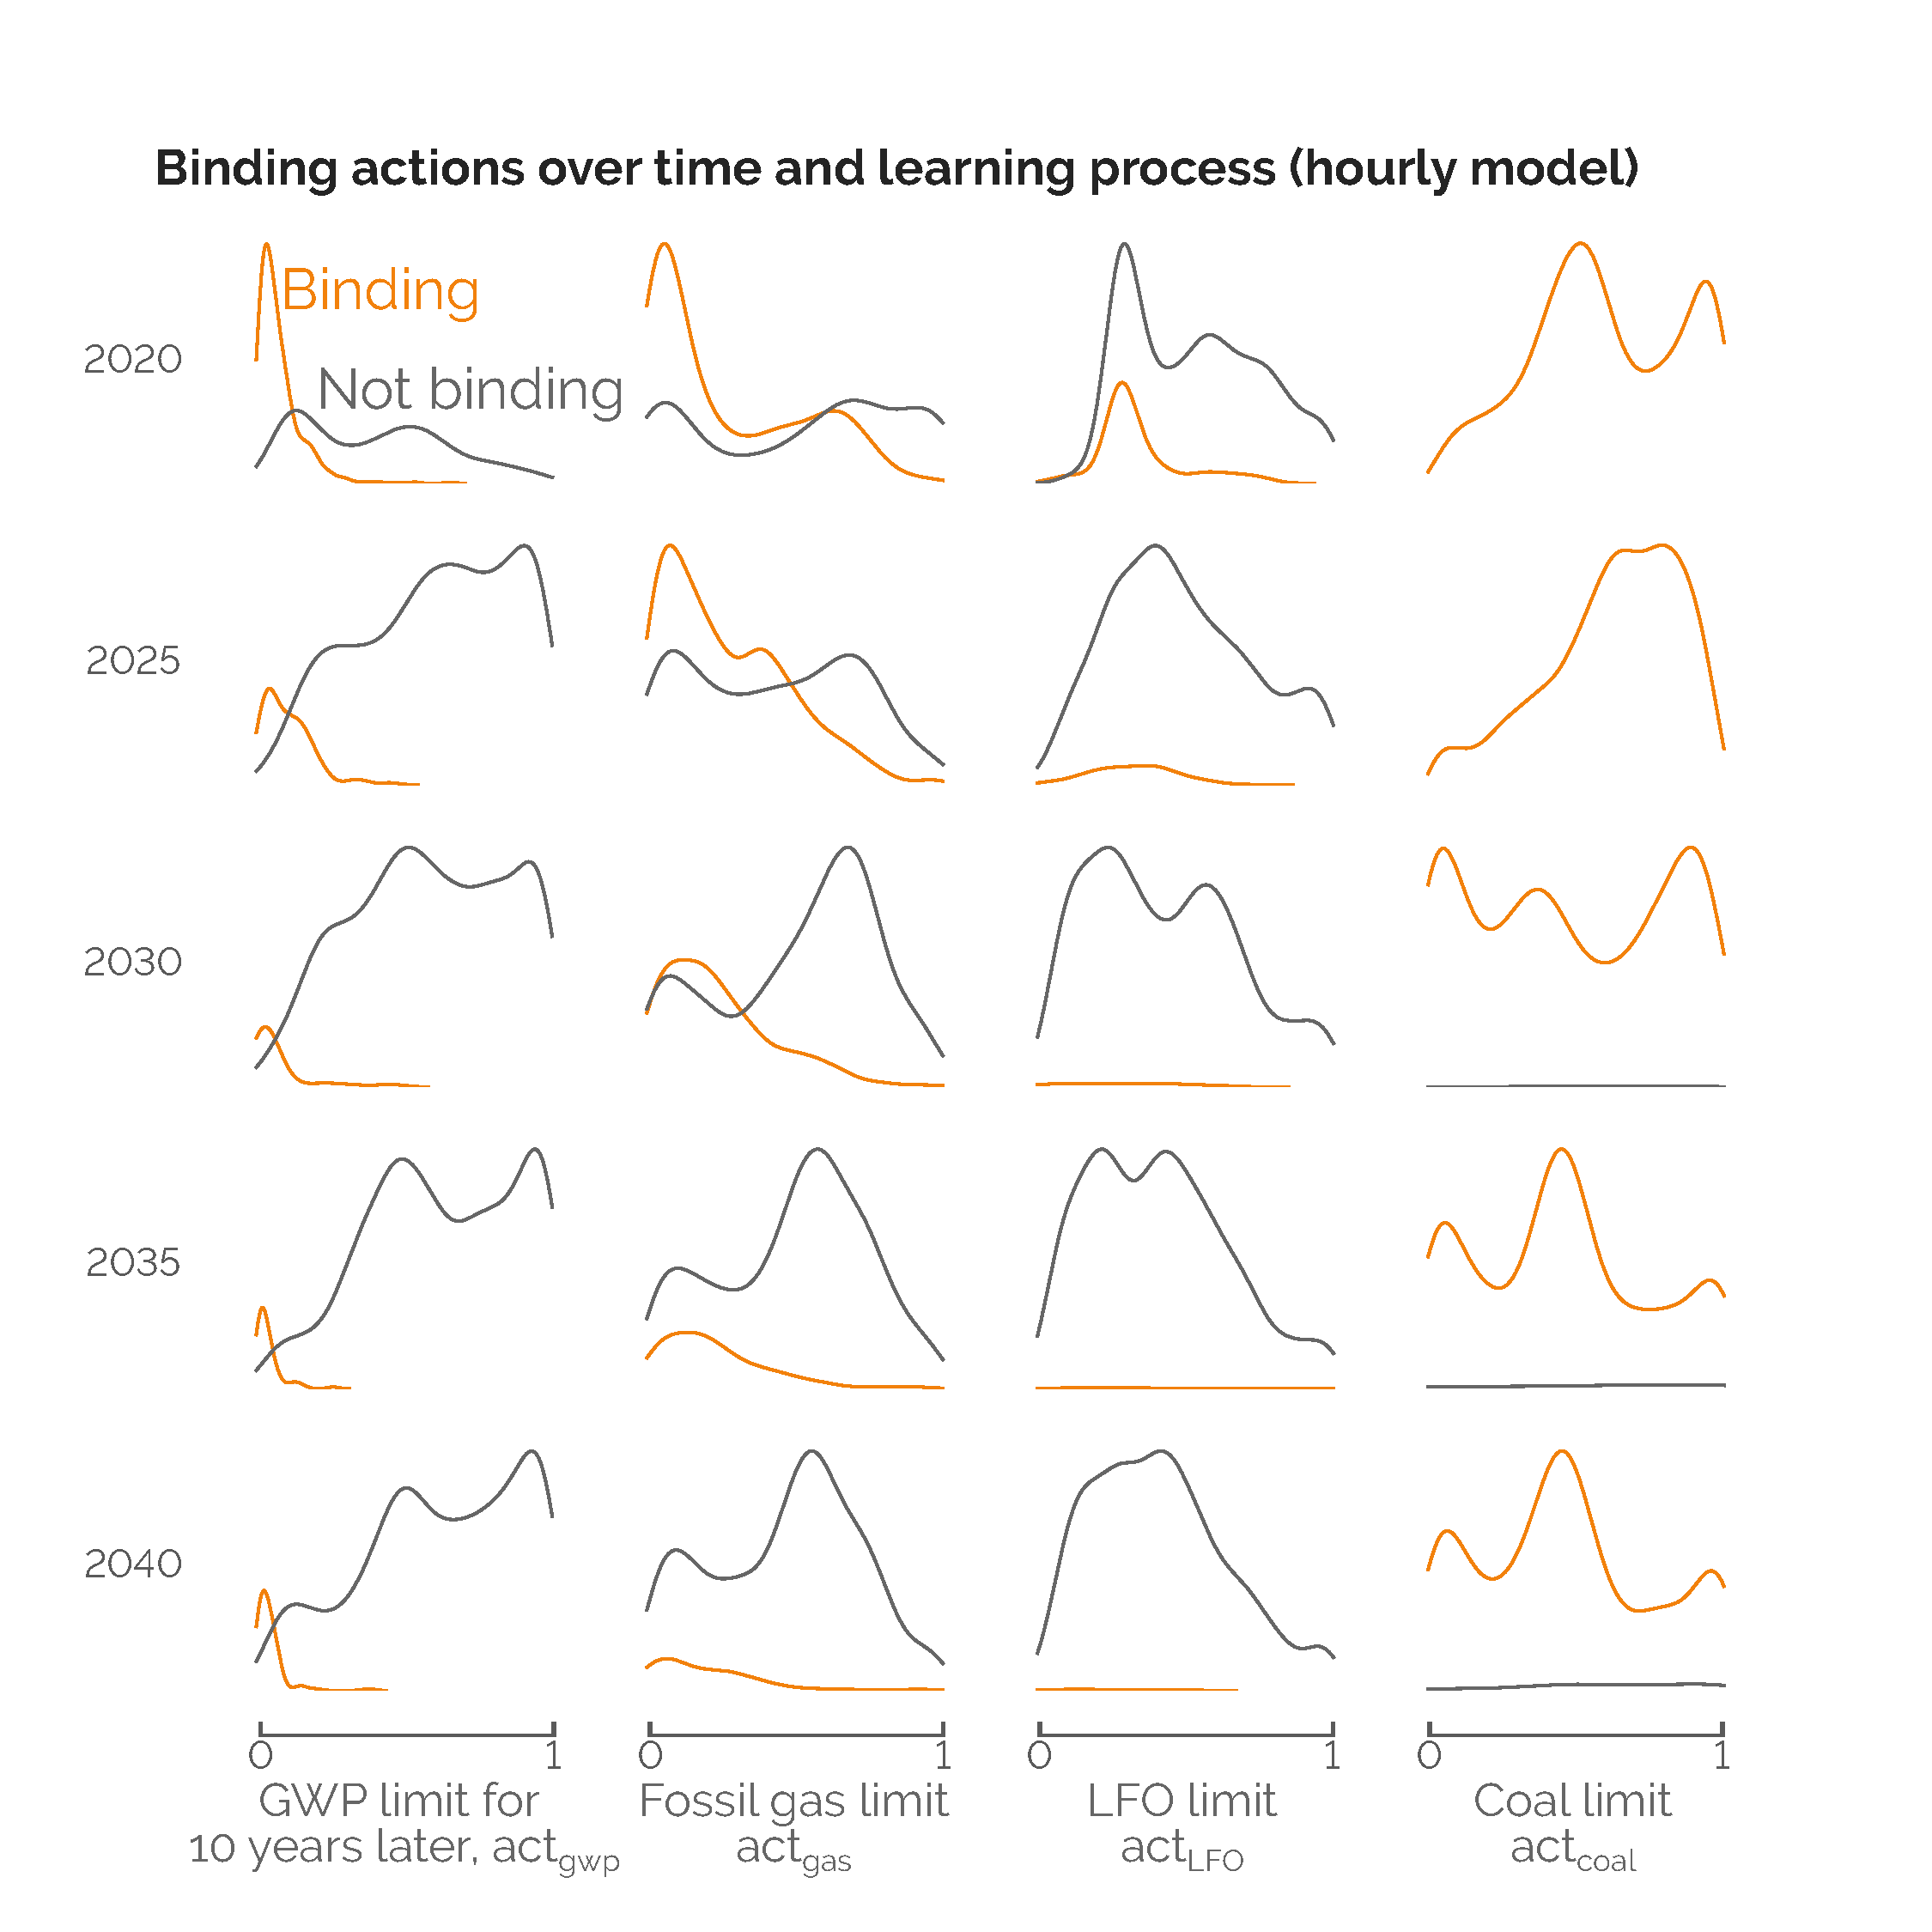
\includegraphics[width=0.49\textwidth]{Binding_learning_TD_joss.pdf}
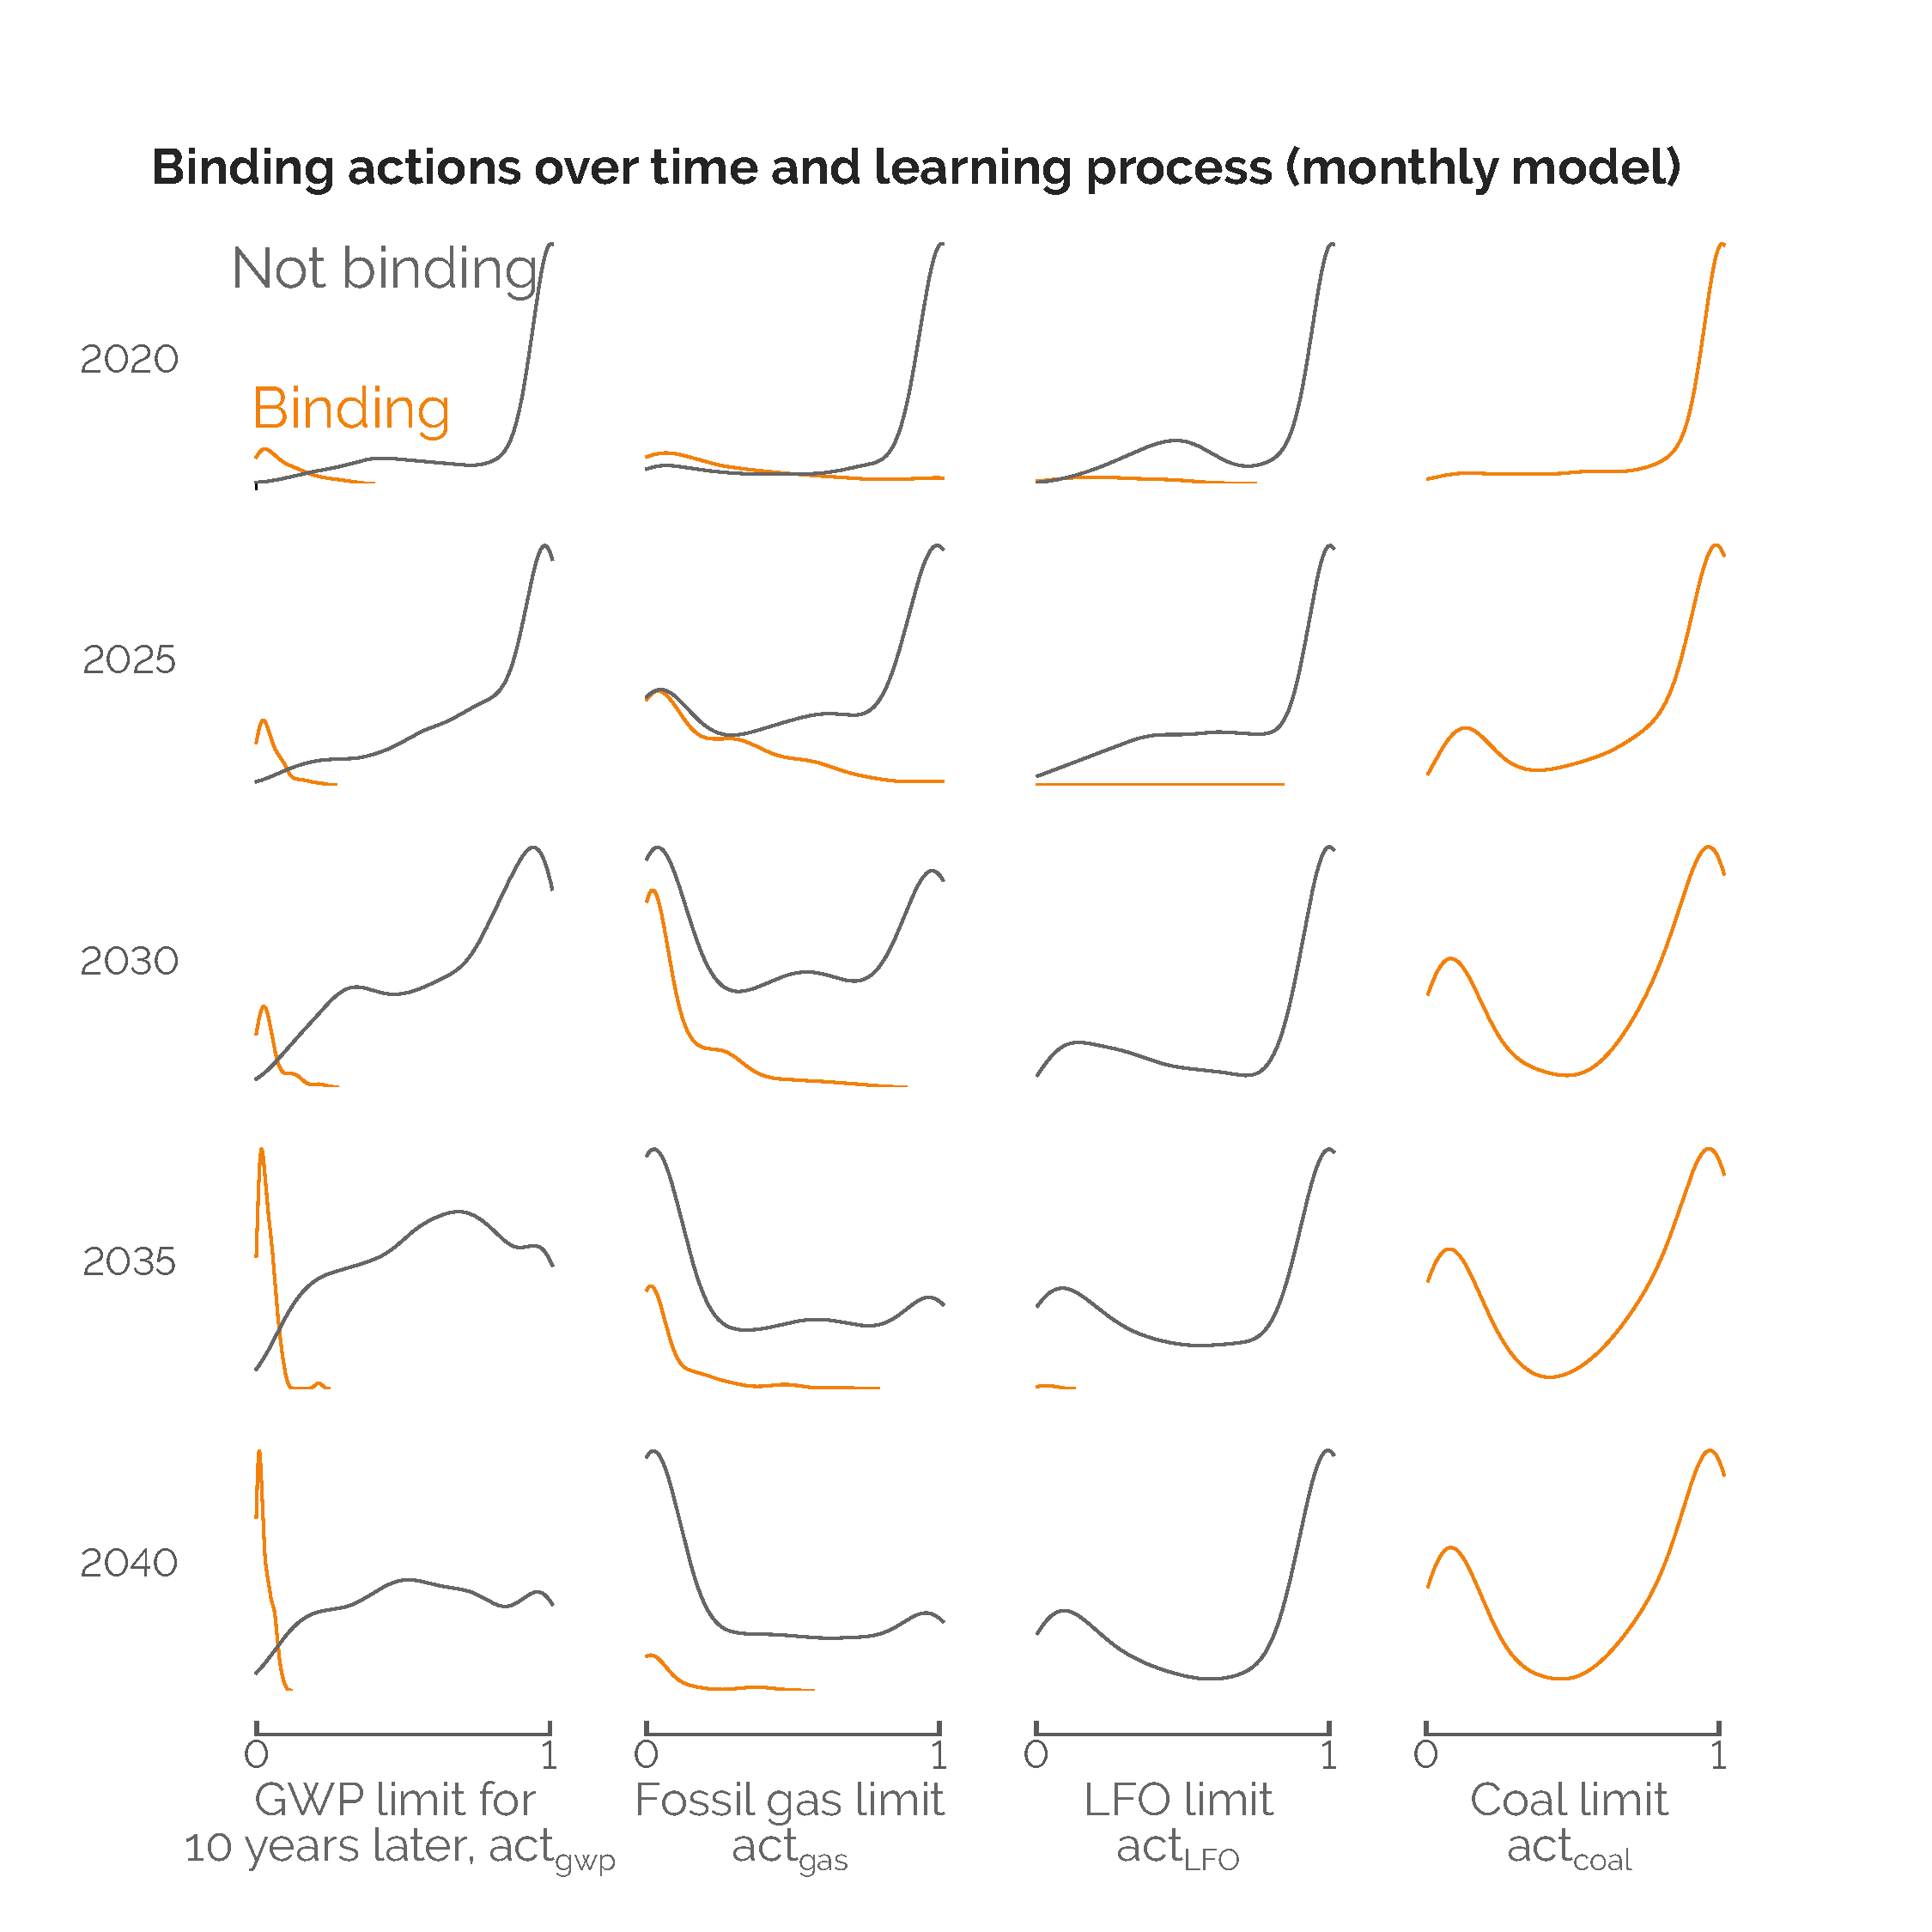
\includegraphics[width=0.49\textwidth]{Binding_learning_MO_joss.pdf}
\caption{Binding versus non-binding constraints on the hourly and monthly models. When the agent learns on the monthly model, the actions are binding in the similar timing and similar ranges as when learning on the hourly model. }
\label{fig:app:Binding_constr_joss}
\end{figure} 

Besides the sharper decrease of emissions early in the transition, the monthly myopic pathways fit with the trend provided by \gls{RL} optimisation on the hourly model. The difference in the early drop of emissions between the monthly and hourly models comes from the easier integration of local \gls{VRES} as the hourly intermittency is averaged over a month (see Appendix \ref{app:mo_vs_td}). 

%\begin{figure}[!htbp]
%\centering
%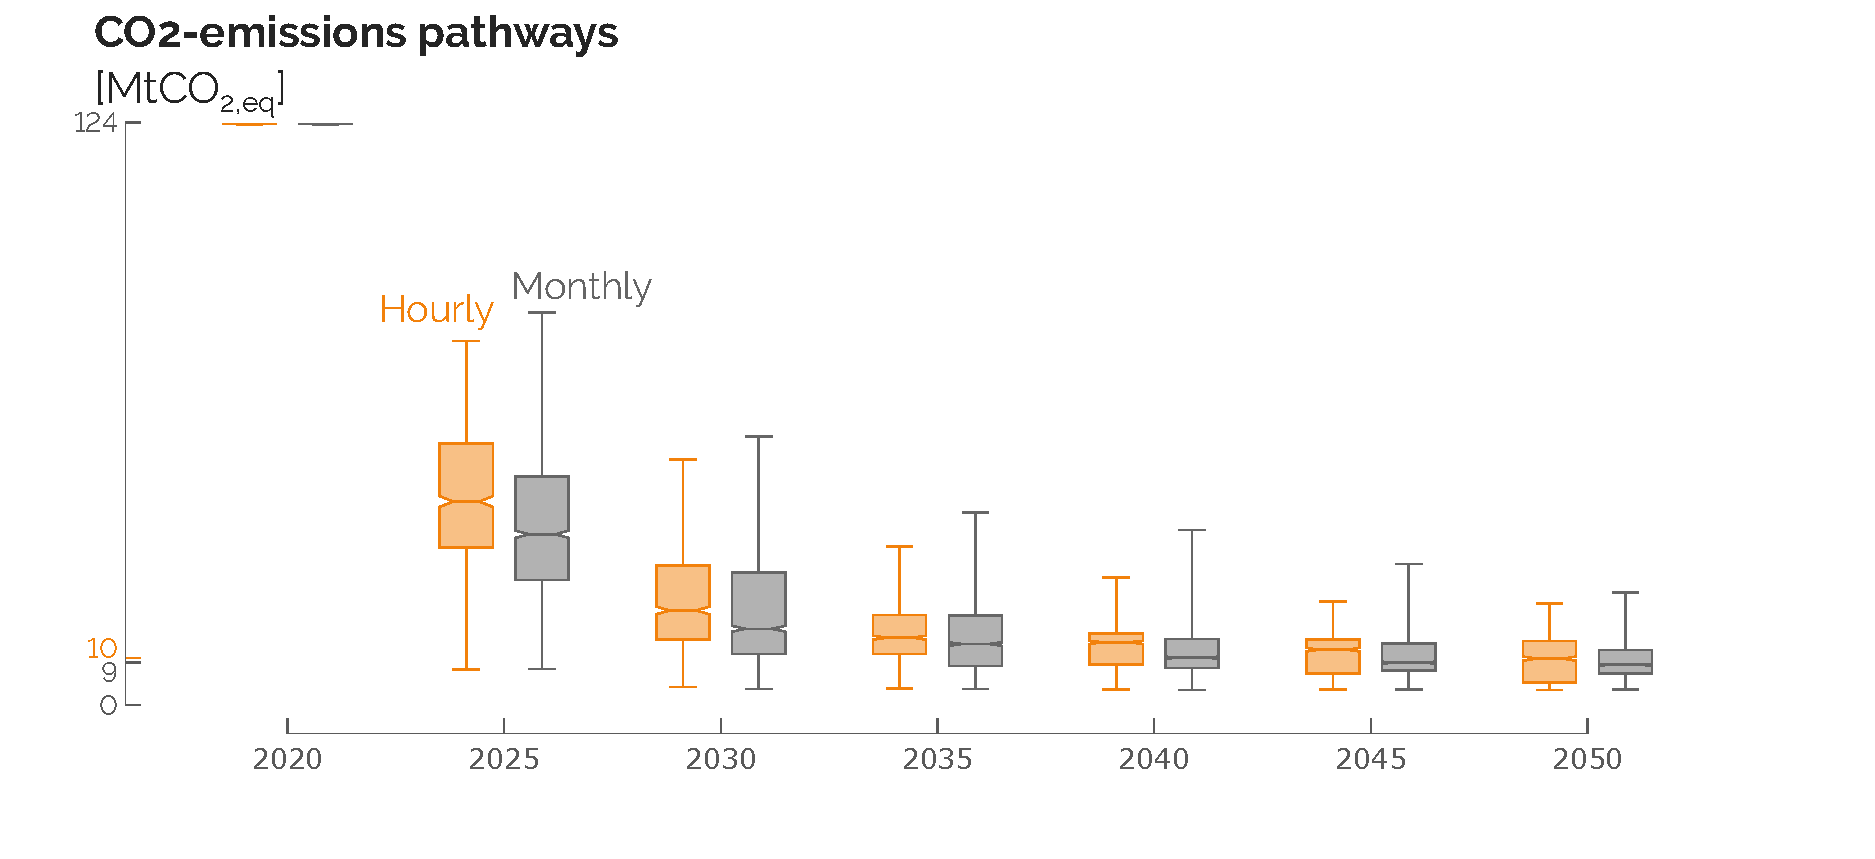
\includegraphics[width=0.8\textwidth]{Gwp_pathway_app.pdf}
%\caption{Comparison of \ce{CO2}-emissions pathways from the \gls{RL}-based myopic optimisation on the hourly and monthly models.}
%\label{fig:app:Gwp_pathway}
%\end{figure}


Even more than for the emissions, the monthly model is a good proxy to assess the pathways of annual system cost as well as cumulative costs such as CAPEX, OPEX and salvage value by 2050 (see Figures \ref{fig:app:System_cost_pathway} and \ref{fig:app:Opex_Capex_Salvage_comp}).

\begin{figure}[!htbp]
\centering
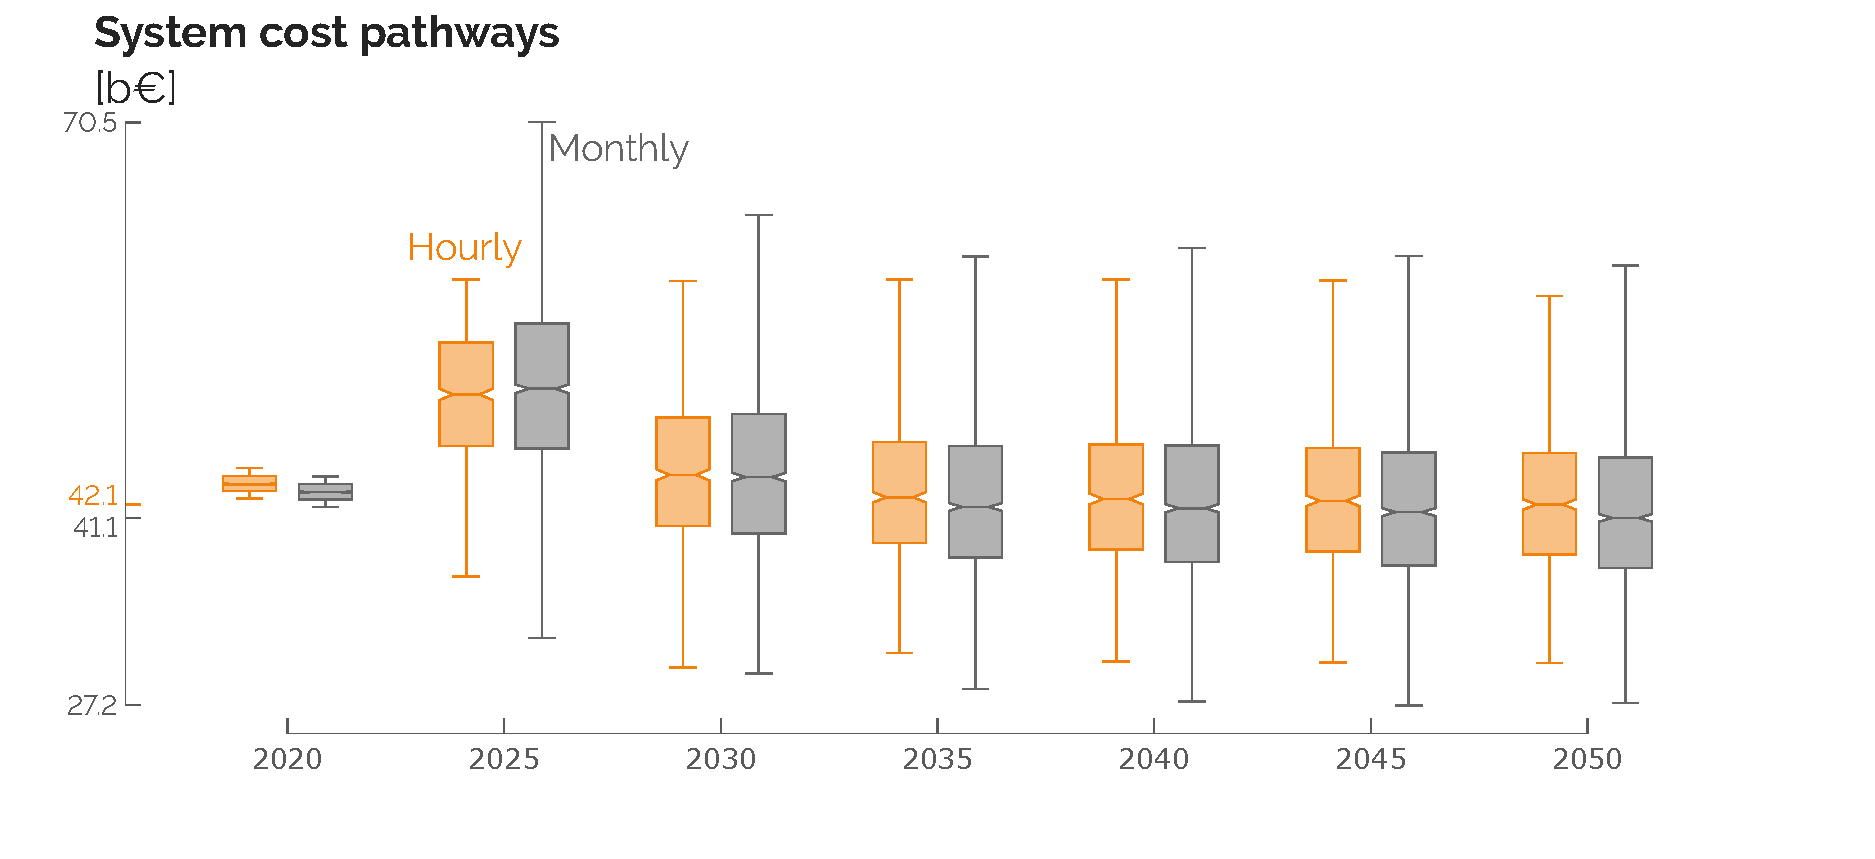
\includegraphics[width=0.8\textwidth]{System_cost_pathway_app.pdf}
\caption{Comparison of annual system cost pathways from the \gls{RL}-based myopic optimisation on the hourly and monthly models.}
\label{fig:app:System_cost_pathway}
\end{figure}

\begin{figure}[!htbp]
\centering
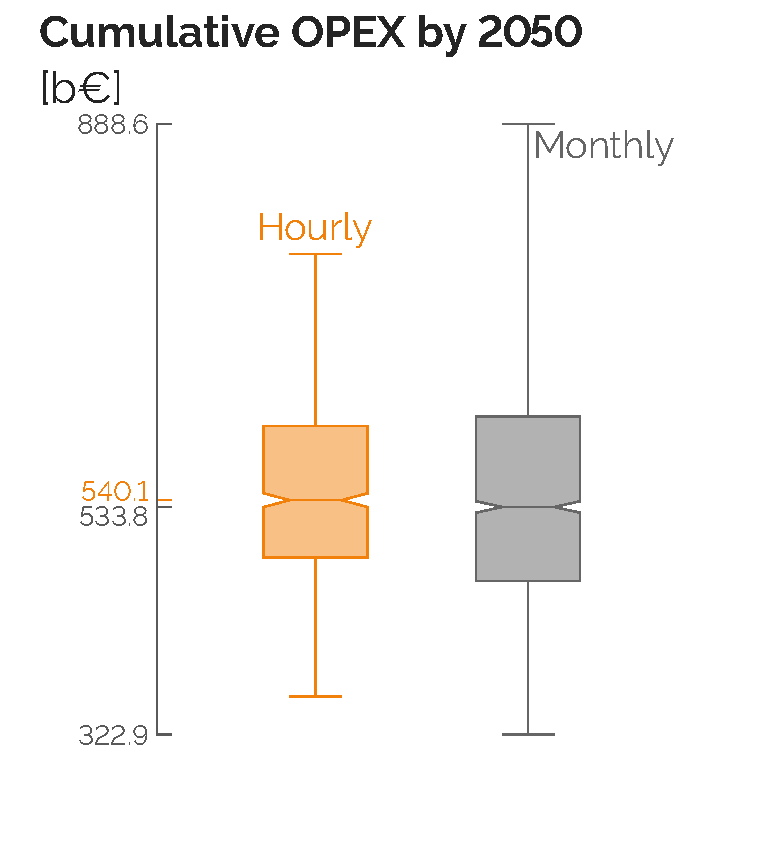
\includegraphics[width=0.325\textwidth]{Opex_2050_comp_app.pdf}
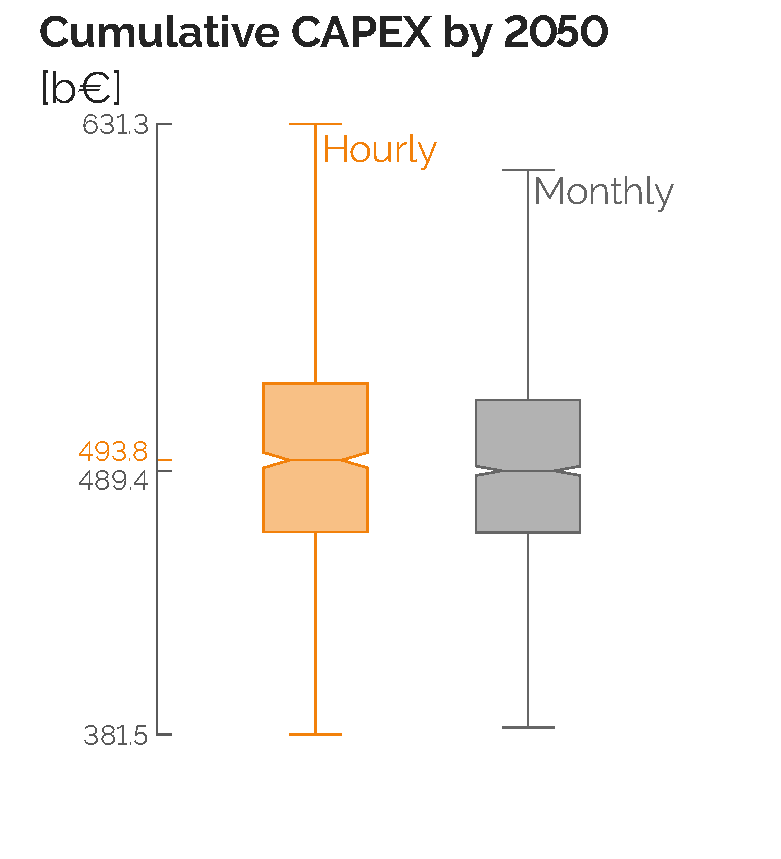
\includegraphics[width=0.325\textwidth]{Capex_2050_comp_app.pdf}
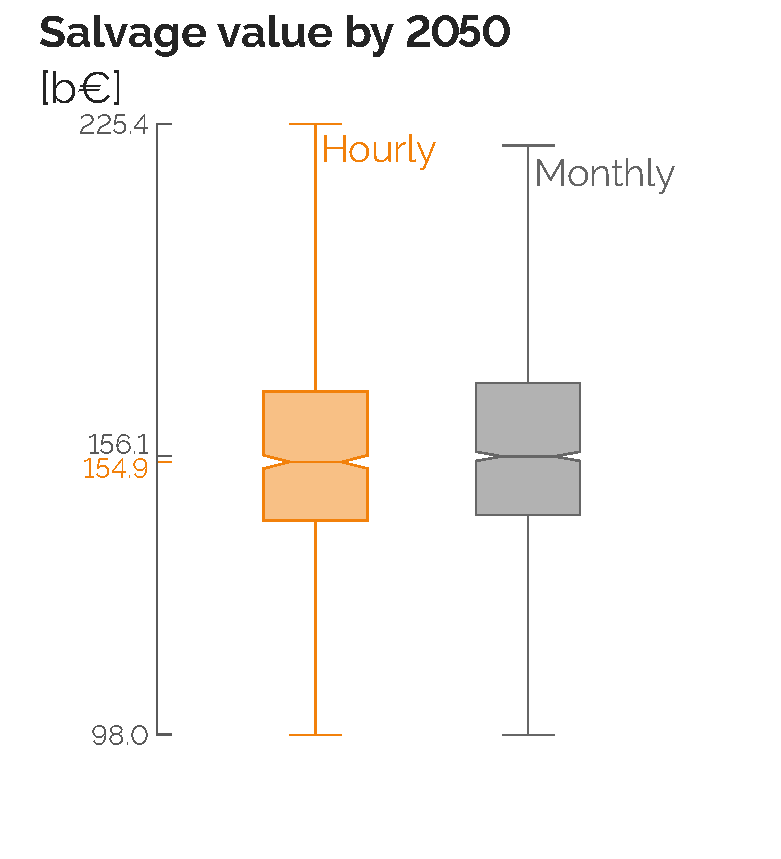
\includegraphics[width=0.325\textwidth]{Salvage_2050_comp_app.pdf}
\caption{Comparison of cumulative OPEX (left), CAPEX (right) and salvage value (right) in 2050 from the \gls{RL}-based myopic optimisation on the hourly and monthly models.}
\label{fig:app:Opex_Capex_Salvage_comp}
\end{figure}

\newpage
The monthly model also captures the need to import more electrofuels by 2050 in the myopic transitions (see Figure \ref{fig:app:Mix_2050_comp}). The other main difference concerns the import of electricity from neighbouring countries. As detailed in Appendix \ref{app:mo_vs_td}, this comes from the averaging of the hourly times series of \gls{VRES} that can provide electricity in a more constant way.

\begin{figure}[!htbp]
\centering
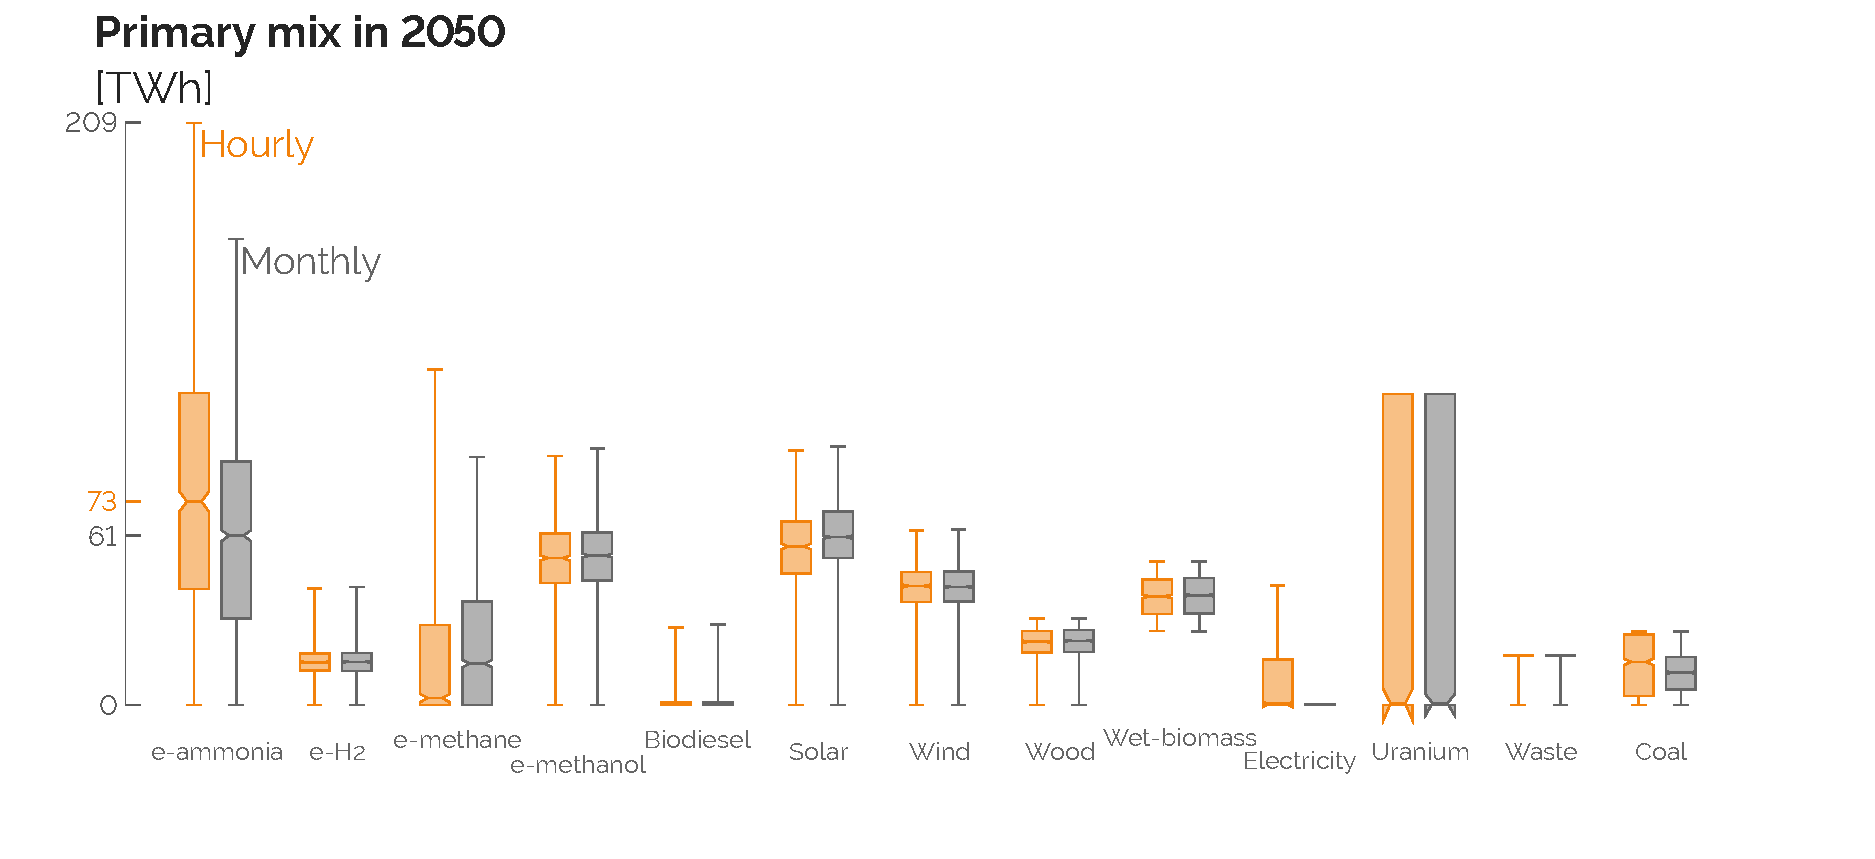
\includegraphics[width=0.8\textwidth]{Mix_2050_comp_app.pdf}
\caption{Comparison of the primary energy mix in 2050 from the \gls{RL}-based myopic optimisation on the hourly and monthly models. To a lesser extent that the hourly model, the monthly optimisation also captures the need to import more electrofuels when the foresight is limited.}
\label{fig:app:Mix_2050_comp}
\end{figure}

In conclusion, with the advantage of the smaller computational burden, the monthly model myopic model is found to be a good proxy with its equivalent based on hourly time-resolution.